\documentclass[twocolumn,aps,prd,floatfix,preprintnumbers,a4paper,nofootinbib,
superscriptaddress,10pt]{revtex4-1}

\usepackage{epsfig}
\usepackage{graphics}
\usepackage{graphicx}
\usepackage{amsmath,amssymb,mathtools}
\usepackage{amsfonts}
\usepackage{bm,soul}
\usepackage[usenames,dvipsnames]{color}
\usepackage{amssymb}
\usepackage{url}
\usepackage{psfrag}
\usepackage{times}
\usepackage[varg]{txfonts}
\usepackage[colorlinks, pdfborder={0 0 0}]{hyperref}
\usepackage{lineno}
\usepackage{verbatim}
\definecolor{LinkColor}{rgb}{0.75, 0, 0}
\definecolor{CiteColor}{rgb}{0.75, 0, 0}
\definecolor{UrlColor}{rgb}{0, 0, 0.75}
\hypersetup{linkcolor=LinkColor}
\hypersetup{citecolor=CiteColor}
\hypersetup{urlcolor=UrlColor}
\usepackage[utf8]{inputenc}
\usepackage{ulem}
\normalem
\hoffset -0.17in
\voffset 0.3in
\textheight 10in

\usepackage{algorithm}
\usepackage{algpseudocode} % in place of algorithmic. Conflicts with revtex4 unless [H] option passed
\usepackage{setspace} % for pleasent spacing in algorithm

%%%%%%%%%%%%%%%%%%%%%%%%%%%%%%%% Useful Definitions %%%%%%%%%%%%%%%%%%%%%%%%%%%%%%%%%%%%%%%%%

% definitions


\usepackage{inputenc}
\usepackage{pgfplots}
\usepackage{tikz}
\usetikzlibrary{shapes,arrows}
\usetikzlibrary{positioning}
\usetikzlibrary{backgrounds}

\def\singleline{
	\begin{center}
	\line(1,0){250}
	\end{center}
}

\newenvironment{aside}
    {\begin{addmargin}[1em]{2em}% 2em left, 1em right
\begin{center} \noindent\rule{0.65\paperwidth}{0.4pt} \end{center}
    }
    {
    \begin{center} \noindent\rule{0.65\paperwidth}{0.4pt} \end{center}
\end{addmargin}
    }

% CUSTOM COMMANDS
\newcommand\xquote[1]{``#1"}
\newcommand\psinr[2]{$\psi_{{#1}{#2}}^{NR}$}
% \newcommand\red[1]{{\color{red} #1}}
\newcommand\red[1]{{\color[rgb]{0.75,0.0,0.0} #1}}
\newcommand\green[1]{{\color[rgb]{0.0,0.60,0.08} #1}}
\newcommand\blue[1]{{\color[rgb]{0,0.20,0.65} #1}}
\newcommand\cyan[1]{{\color[HTML]{00c3ff} #1}}
\newcommand\bluey[1]{{\color[rgb]{0.11,0.20,0.4} #1}}
\newcommand\gray[1]{{\color[rgb]{0.7,0.70,0.7} #1}}
\newcommand\grey[1]{{\color[rgb]{0.7,0.70,0.7} #1}}
\newcommand\white[1]{{\color[rgb]{1,1,1} #1}}
\newcommand\darkgray[1]{{\color[rgb]{0.3,0.30,0.3} #1}}
\newcommand\orange[1]{{\color[rgb]{.86,0.24,0.08} #1}}
\newcommand\purple[1]{{\color[rgb]{0.45,0.10,0.45} #1}}
\newcommand\note[1]{\colorbox[rgb]{0.85,0.94,1}{\textcolor{black}{\textsc{\textsf{#1}}}}}

%
\newcommand*{\figfactor}{0.495}

% Math symbols
% ###################################### %
%\def\mh{{\hat{h}}} % model  for strain
\def\m#1{{\hat{#1}}} % model  for strain
\def\ma#1{{\hat{#1}_{\bm{a}}}} % model  for strain
\newcommand{\var}[1]{\mathcal{{#1}}}
\newcommand{\mlam}{{\bm{\lambda}}}
\newcommand{\lam}{{\lambda}}
\newcommand{\mLam}{{\bm{\Lambda}}}
\newcommand{\bigo}[1]{{\cal O}({#1})}
\newcommand{\braket}[2]{ {\langle {#1} | {#2} \rangle} }
% ###################################### %

% ###################################### %
\definecolor{lightblue}{rgb}{.82,.88,0.95}
\definecolor{lightred}{rgb}{0.95,.86,0.86}
\definecolor{yellow}{rgb}{0.95,0.95,0.86}
\definecolor{green}{rgb}{.90,1,0.95}
\definecolor{lightpurple}{rgb}{.95,0.85,0.95}
% ###################################### %

\tikzset{
    vertex/.style = {
        circle,
        fill            = black,
        outer sep = 2pt,
        inner sep = 1pt,
    }
}


% CUSTOM DEFINITIONS
% ***************************************** %
\def\prd{Phys.Rev.D}
% ***************************************** %
\def\gt{Georgia Tech}
% ***************************************** %
\def\tk{Teukolsky}
% ***************************************** %
\def\mp{multipole}
% ***************************************** %
\def\ee{Einstein's equations}
% ***************************************** %
\def\toolkit#1{NRDA--Toolkit{#1}}
% \def\toolkit#1{Data Analysis Toolkit{#1}}
% ***************************************** %
\def\wf#1{waveform#1}
% ***************************************** %
\def\grad#1{gravitational radiation#1}
% ***************************************** %
\def\gr#1{General Relativity#1}
% ***************************************** %
\def\gwa#1{Gravitational Wave Astrophysics#1}
% ***************************************** %
\def\gwf#1{gravitational waveform#1}
% ***************************************** %
\def\gw#1{gravitational wave#1}
% ***************************************** %
\def\gwa#1{\gw{} astronomy#1}
% ***************************************** %
\def\nht#1{No-Hair Theorem#1}
% ***************************************** %
\def\rm#1{\mathrm{#1}}
% ***************************************** %


% Referencing
% ***************************************** %
\def\prt#1{Part~(\ref{#1})}
% ***************************************** %
\def\ap#1{Appendix~(\ref{#1})}
% ***************************************** %
\def\ch#1{Chapter~(\ref{#1})}
% ***************************************** %
\def\cch#1{Chapter~\ref{#1}}
% ***************************************** %
\newcommand{\chs}[2]{Chapters~(\ref{#1}-\ref{#2})}
% ***************************************** %
\newcommand{\cchs}[2]{Chapters~\ref{#1}-\ref{#2}}
% ***************************************** %
\def\sec#1{Section~(\ref{#1})}
% ***************************************** %
\def\csec#1{Section~\ref{#1}}
% ***************************************** %
\def\tk#1{Teukolsky#1}
% ***************************************** %
\newcommand{\secs}[2]{Sections~(\ref{#1}-\ref{#2})}
% ***************************************** %
\def\fig#1{Fig.~\ref{#1}} % NOTE that PRL requires that Fig. be used rather
% than figure
% \def\fig#1{\hyperref[#1]{Figure~\ref{#1}}}
% ***************************************** %
\def\cfig#1{Fig.~\ref{#1}}
% \def\cfig#1{Figure~\ref{#1}}
% ***************************************** %
\newcommand{\figs}[2]{Figures~(\ref{#1}-\ref{#2})}
% ***************************************** %
\def\eqn#1{Eqn.~(\ref{#1})}
% \def\eqn#1{Equation~(\ref{#1})}
% ***************************************** %
\def\ceqn#1{Eqn.~\ref{#1}}
% \def\ceqn#1{Equation~\ref{#1}}
% ***************************************** %
\newcommand{\eqns}[2]{Equations~(\ref{#1})--(\ref{#2})}
% ***************************************** %
\newcommand{\ceqns}[2]{Equations~\ref{#1}--\ref{#2}}
% ***************************************** %
\def\tbl#1{Table~(\ref{#1})}
% ***************************************** %
\def\ctbl#1{Table~\ref{#1}}
% ***************************************** %


% ***************************************** %
\def\da#1{data analysis#1}
% ***************************************** %
\def\imr#1{inspiral, merger and ringdown#1
  (IMR#1)\gdef\imr{IMR}}
% ***************************************** %
\def\lal#1{LIGO Analysis Library#1
  (LAL#1)\gdef\lal{LAL}}
% ***************************************** %
\def\nrda#1{\nr{} Data Analysis#1
  (NRDA#1)\gdef\nrda{NRDA}}
% ***************************************** %
\def\tt#1{\textit{transverse--traceless}#1
  (TT#1)\gdef\tt{TT}}
% ***************************************** %
\def\et#1{Einstein Telescope#1
  (ET#1)\gdef\et{ET}}
% ***************************************** %
\def\ego#1{European Gravitational Observatory#1
  (EGO#1)\gdef\ego{EGO}}
% ***************************************** %
\def\elisa#1{Evolved Laser Interferometer Space Antenna#1
  (eLISA#1)\gdef\elisa{eLISA}}
% ***************************************** %
\def\ligo#1{Laser Interferometer Gravitational Wave Observatory#1
  (LIGO#1)\gdef\ligo{LIGO}}
% \def\ligo#1{LIGO#1}
% ***************************************** %
\def\virgo#1{Virgo#1}
% ***************************************** %
\def\aligo#1{Advanced LIGO#1
  (aLIGO#1)\gdef\aligo{aLIGO}}
% ***************************************** %
\def\snr#1{signal-to-noise ratio#1
  (SNR#1)\gdef\snr{SNR}}
% ***************************************** %
\def\psd#1{power spectral density#1
  (PSD#1)\gdef\psd{PSD}}
% ***************************************** %
\def\rom#1{reduced order model#1
  (ROM#1)\gdef\rom{ROM}}
% ***************************************** %
\def\gatech#1{Georgia Institute of Technology#1
  (GaTech#1)\gdef\gatech{GaTech}}
% ***************************************** %
\def\ffi#1{Fixed-Frequrncy Integration#1
  (FFI#1)\gdef\ffi{FFI}}
% ***************************************** %
\def\sxs#1{Simulating Extreme Spacetimes#1
  (SXS#1)\gdef\sxs{SXS}}
% ***************************************** %
\def\bam#1{Bifunctional Adaptive Mesh#1
  (BAM#1)\gdef\bam{BAM}}
% ***************************************** %
\def\adm#1{Arnowitt-Deser-Misner
	(ADM#1)\gdef\adm{ADM}}
%
\def\frmse#1{Fractional Root-Mean Square Error
	(FRMSE)\gdef\frmse{FRMSE}}


% ***************************************** %
\def\bh#1{black hole#1
 (BH#1)\gdef\bh{BH}}
% \def\bh#1{black hole#1}
% ***************************************** %
%\def\bbh#1{binary black hole#1
%  (BBH#1)\gdef\bbh{BBH}}
\def\bbh#1{binary \bh{}#1}
% ***************************************** %
\def\bhb#1{\bh{} binary#1}
% ***************************************** %


% ***************************************** %
\def\qnm#1{Quasi-Normal Mode#1
  (QNM#1)\gdef\qnm{QNM}}
% ***************************************** %
\def\eob#1{Effective One Body#1
  (EOB#1)\gdef\eob{EOB}}
% ***************************************** %
\def\gw#1{gravitational-wave#1}
\def\gw#1{Gravitational wave#1
 (GW#1)\gdef\gw{GW}}
% ***************************************** %
\def\gwa#1{gravitational wave astronomy#1}
% ***************************************** %
\def\spa#1{stationary phase approximation#1
 (SPA#1)\gdef\spa{SPA}}
% ***************************************** %
\def\pn#1{Post-Newtonian#1
	(PN#1)\gdef\pn{PN}}
% ***************************************** %
\def\pnl#1{post-Newtonian-like#1
  (PN-like#1)\gdef\pnl{PN-like}}
% ***************************************** %
% \def\nr{Numerical Relativity}
\def\NR{{\text{NR}}}
\def\nr{Numerical Relativity
 (NR)\gdef\nr{NR}}
% ***************************************** %
\def\pt{perturbation theory}
% ***************************************** %
\def\GOLS#1{\textit{greedy ordinary least-squares}#1}
% ***************************************** %
\def\rd{ringdown}
% ***************************************** %
% \def\imr{inspiral, merger and \rd{}}
% ***************************************** %
\def\cbc#1{compact object coalescence#1}
% ***************************************** %
\def\bbc#1{binary black hole coalescence#1}
%\def\bbc#1{binary black hole coalescence#1
%  (BBC#1)\gdef\bbc{BBC}}
% ***************************************** %
\def\pc#1{principle component#1}
% ***************************************** %
\def\pca#1{principle component analysis#1
  (PCA#1)\gdef\pca{PCA}}
% ***************************************** %
\def\svd#1{Singular Value Decomposition#1
  (SVD#1)\gdef\svd{SVD}}
% ***************************************** %
\def\gs#1{Gram-Schmidt#1}
% ***************************************** %
% ***************************************** %
\newcommand*{\factor}{0.95} % for figure scale
\newcommand*{\rscale}{1.3}
% ***************************************** %

% ******************************************************* %
\def\study{work} %
% ******************************************************* %

\newcommand{\osum}{\operatornamewithlimits{
\hspace{-2pt}{\bigcup\hspace{-9.5pt}\circ}
}}

% commutative multiplication
\newcommand{\ox}{\operatornamewithlimits{
{\circ\hspace{-3.7pt}\cdot}
}}

% non-commutative multiplication
\newcommand{\cc}{ \circledcirc }

% general subtraction
\newcommand{\om}{ \mathrel{\raisebox{1pt}{$\scriptscriptstyle\circleddash$}} }






\newcommand{\hlgreen}[1]{\sethlcolor{green}\hl{#1}{\sethlcolor{yellow}}}
\newcommand{\hlyellow}[1]{\sethlcolor{yellow}\hl{#1}{\sethlcolor{yellow}}}
\newcommand{\hlblue}[1]{\sethlcolor{lightblue}\hl{#1}{\sethlcolor{yellow}}}
\newcommand{\hlred}[1]{\sethlcolor{lightred}\hl{#1}{\sethlcolor{yellow}}}
\newcommand{\hlpurple}[1]{\sethlcolor{lightpurple}\hl{#1}{\sethlcolor{yellow}}}

\newcommand{\hlbackground}[1]{\sethlcolor{green}\hl{#1}{\sethlcolor{yellow}}}
\newcommand{\hlproblem}[1]{\sethlcolor{yellow}\hl{#1}{\sethlcolor{yellow}}}
\newcommand{\hlmethods}[1]{\sethlcolor{lightblue}\hl{#1}{\sethlcolor{yellow}}}
\newcommand{\hlresults}[1]{\sethlcolor{lightred}\hl{#1}{\sethlcolor{yellow}}}
\newcommand{\hldiscussion}[1]{\sethlcolor{lightpurple}\hl{#1}{\sethlcolor{yellow}}}


% Richard's stuff

\newcommand\aap{\&A}
\newcommand\apss{APSS}
\newcommand\aaps{AAPS}
\newcommand\apjs{ApJ S}
\newcommand\aj{AJ}
\newcommand\apjl{ApJL}
\newcommand\mnras{MNRAS}
\newcommand\pasp{PASP}
\newcommand\araa{ARAA}
\newcommand\physrep{Phys. Rep.}

\newcommand\nrRequest{\textbf{NR INPUT?}}
\newcommand\richardBugFix{\textbf{\color{red}Richard will bugfix}}
\newcommand\editremark[1]{ {\color{red} #1}}
\newcommand\newtext[1]{{\bf #1}}
\newcommand\recentlychanged[1]{{\bf #1}}
\newcommand\hidetosubmit[1]{}
%
\newcommand\optional[1]{}
\newcommand\ForInternalReference[1]{}
\newcommand\embrace[1]{{[#1]}}
\newcommand\unit[1]{\, {\rm #1}}
\newcommand\mc{ {{\cal M}_c}}
\newcommand\Dho{ {D_{\rm H}^{(0)}}}
\newcommand\Dh{ {D_{\rm H}}}
\newcommand\Deff{{D_{\rm eff}}}  %
\newcommand\Dv{{D_{\rm v}}}      %
\newcommand\Dc{{D_c}}            %
\newcommand\Y[1]{Y^{(#1)}}


\newcommand\avL{\left< {\cal L}_{(a} {\cal L}_{b)} \right>}
\newcommand\WeylScalar{{\psi_4}}
\newcommand\WeylScalarFourier{{\tilde{\psi}_4{}}}
\newcommand\FourierWeylScalar{{\tilde{\psi}_4}}
\newcommand\WeylScalarCorot{R^{-1}{\psi_4}}

\newcommand\qmstate[1]{\left|#1\right>}
\newcommand\qmstateKet[1]{\left<#1\right|}
\newcommand\qmstateproduct[2]{\left<#1|#2\right>}
\newcommand\qmoperatorelement[3]{\left<#1\left|#2\right|#3\right>}
\newcommand\qmoperator[1]{{\bf #1}}
\newcommand\myvector[1]{{\mathbf{#1}}}
\newcommand\chip{{\boldsymbol{\chi}_+}}
\newcommand\chim{{\boldsymbol{\chi}_-}}

\newcommand\nSimulationsTotal{224}   %
\newcommand\nSimulationsNonprecessing{62}  %
\newcommand\ReferenceMassLow{100}      %
\newcommand\ReferenceMassMiddle{300}   %
\newcommand\ReferenceMassHigh{1000}   %


\newcommand\abbrvPSgrbs{PS-GRB}
\newcommand\abbrvCBC{CBC}

\def\check#1{\red{#1}}
\def\remove#1{\hlred{#1}}
\newcommand{\cw}{\tilde{\omega}}
\newcommand{\CW}{\tilde{\Omega}}
\newcommand{\CWr}{{\Omega}^{\mathrm{r}}}
\newcommand{\CWc}{{\Omega}^{\mathrm{c}}}
\newcommand{\SC}{\mathcal{K}}
\newcommand{\CC}{\mathcal{C}}
\newcommand{\SCr}{\mathcal{K}^{\mathrm{r}}}
\newcommand{\SCc}{\mathcal{K}^{\mathrm{c}}}
\newcommand{\lalapprox}{\texttt{MMRDNS}}
\def\jf{j_f}
\def\mf{M_f}
\newcommand{\LL}{\bar{l}}
\newcommand{\MM}{\bar{m}}
\def\lmn{_{\ell m n}}
\def\LM{_{\bar{\ell} \bar{m}}}
\def\LMlmn{_{\bar{\ell} \bar{m} \ell m n}}
\def\gmvp#1{greedy-multivariate-polynomial#1
  (\texttt{GMVP}#1)\gdef\gmvp{\texttt{GMVP}}}
\def\gmvr#1{greedy-multivariate-rational#1
  (\texttt{GMVR}#1)\gdef\gmvr{\texttt{GMVR}}}

\newcommand{\lmtitle}[2]{\vspace{-0.80cm} \begin{center} \noindent\rule{0.35\paperwidth}{0.3pt} \end{center} \vspace{-0.3cm}}

% Numbers that may change from time to time
\def\CwFitCalibrationRegion{\red{0.995} }
\def\NumCalibrationPointsPlotted{\red{21} }
\def\NumCalibrationPoints{\red{61} }

%%%%%%%%%%%%%%%%%%%%%%%%%%%%%%%%%%%%%%%%%%%%%%%%%%%%%%%%%%%%%%%%%%%%%%%%%%%%%%%%%%%%%%%%%%%%%

\begin{document}

%%%%%%%%%%%%%%%%%%%%%%%%%%%%%%%%%%%%%% Title page %%%%%%%%%%%%%%%%%%%%%%%%%%%%%%%%%%%%%%%%%%%

\title{Notes on modeling for Kerr black holes: Basis learning, QNM frequencies, and spherical-spheroidal mixing coefficients }

\author{L. London}
\affiliation{School of Physics and Astronomy, Cardiff University, The Parade, Cardiff, CF24 3AA, United Kingdom}

%%%%%%%%%%%%%%%%%%%%%%%%%%%%%%%%%%%%% Abstract %%%%%%%%%%%%%%%%%%%%%%%%%%%%%%%%%%%%%%%%
\begin{abstract}
	%
	The ongoing direct detection of gravitational wave signals is aided by representative models of theoretical predictions. In particular, the process of model based detection, and subsequent comparison of signals the general relativity's predictions are aided by the modeling of information related to perturbed Kerr black holes. Here, we summarize recent methods and models for the analytically understood gravitational wave spectra (quasi-normal mode frequencies), and harmonic structure of Kerr black holes (mixing coefficients between spherical and spheroidal harmonics). Towards the construction of these models, two algorithms, GMVP and GMVR, for the automated polynomial and rational modeling of general dimensional complex scalars are presented.
	%
\end{abstract}
%%%%%%%%%%%%%%%%%%%%%%%%%%%%%%%%%%%%%%%%%%%%%%%%%%%%%%%%%%%%%%%%%%%%%%%%%%%%%%%%%%%%%%%%

%%%%%%%%%%%%%%%%%%%%%%%%%%%%%%%%%%%% Preprint numbers %%%%%%%%%%%%%%%%%%%%%%%%%%%%%%%%%%
%\preprint{LIGO-P1500185-v10}
\date{\today}
%%%%%%%%%%%%%%%%%%%%%%%%%%%%%%%%%%%%%%%%%%%%%%%%%%%%%%%%%%%%%%%%%%%%%%%%%%%%%%%%%%%%%%%%

\maketitle

% \begin{itemize}
% 	\item BH detections happen, and use fits at various levels
% 	\item Fits for Kerr are important for modeling and testing GR, they are fast to eval comapred to formal calculations which has data analysis implications
% 	\item Many fits have been done for perturbative Kerr parameters: QNM frequencies most prominently.
% 	\item The problem/motivation:
% 		\begin{itemize}
% 			\item 1. There are many fits, and we would like to provide a reference for many of them, including key methods
% 			\item 2. Methods for fits: basis learning
% 			\item 3. (results) Summarize "simple fits": QNM frequencies and decay times, enforcing zero damping
% 			\item 4. (results) Summarize more general fits: mixing coefficients
% 		\end{itemize}
% 	\item (discussion) We have presented ...
% \end{itemize}

\section{Introduction}
%
In the coming years, expectations for frequent \gw{} detections of increasing \snr{} are high.
%
Concurrent with \virgo{}, the \aligo{} detectors will enter their third observing run in \check{late 2018}.
%
At this time, \bbh{} detections are expected at a rate of \check{X} per month.
%
In this context, signal detection and subsequent inference of physical parameters hinges upon efficient models for source properties and dynamics.
%
Most prominently, there is ongoing interest in signal models for \bbh{} \imr{}.
%
As the merger of isolated \bh{s} is expected to result in a perturbed Kerr \bh{}, there is related interest in having computationally efficient models for perturbative parameters, namely those that enable evaluation of the related \rd{} radiation.
%
\par In particular, a perturbed Kerr \bh{} (e.g. resulting from \bbh{} merger) will have \gw{} radiation that rings down with characteristic frequencies,
%
$%\begin{align}
	\cw\lmn = \omega\lmn + i/\tau\lmn
$%\end{align}
.
%
These discrete frequencies have associated radial and spatial functions which are \textit{spheroidal} harmonic in nature.
%
These frequencies and harmonic functions are the so-called \qnm{s}.
%
They are the eigen-solutions of the source free linearized \ee{} (i.e. \tk{'s} equations) for a perturbed \bh{} with final mass, $\mf$, and dimensionless final spin, $\jf$.
%
The well known and effective completeness of these solutions allows \grad{} from generic perturbations to be well approximated by a spectral (multipolar) sum which combines the complex \qnm{} amplitude, $A\lmn$, with the spin weight -2 spheroidal harmonics, $_{-2}S\lmn$.
%
\begin{align}
	%
	\label{hrd}
	%
	h &= h_{+} - i \, h_{\times}
	  \\ \nonumber
	  &= \frac{1}{r} \sum\lmn A\lmn \; e^{i\,\cw\lmn t} \; _{-2}S\lmn( \jf \cw\lmn,\theta,\phi)
		\\ \nonumber
		&= \frac{1}{r} \sum\LM h\LM(t) \; _{-2}Y\LM(\theta,\phi) \;  .
	%
\end{align}
%
\par In the first and second lines of \eqn{hrd}, we relate the observable \gw{} polarizations, $h_+$ and $h_\times$, with the analytically understood morphology of the time domain waveform.
%
Here, the labels $\ell$ and $m$ are eigenvalues of \tk{'s} angular equations, where units of $M=1$ (e.g. the initial mass of the \bbh{} system), and $c=1$.
%
In the third line of \eqn{hrd}, we represent $h$ in terms of \textit{spherical} harmonic multipoles.
%
This latter form is ubiquitous for the development and implementation of \imr{} signal models for \bbh{s}.
%
%
\par Towards the development of these models, \eqn{hrd} enters in many incarnations.
%
In the \eob{} formalism, $h\LM$ is modeled such that, after its peak (near merger), the effective functional form reduces (asymptotically) to \eqn{hrd}'s second line.
%
This view currently comes with the added assumption that ${_{-2}}S_{\ell m n} = {_{-2}}Y_{\ell m}$, where only $n=0$ is explicitly considered.
%
The consequences of this choice are discussed in reference \check{[X]}.
%
For the so-called \textit{Phenom} models, the frequency domain multipoles, $\tilde{h}\LM(f)$, are constructed such that their high frequency behavior is consistent with \eqn{hrd} in the time domain.
%
\par Both Phenom and \eob{} approaches directly use phenomenological models (i.e. fits) for the \qnm{} frequencies, as these fits are more computationally efficient than the underlying analytic calculations, which involve the solving of continued fraction equations.
%
In the case of \texttt{PhenomHM} and derivative models, fits for the \qnm{} frequencies are used in the process of mapping $\tilde{h}_{22}(f)$ into other $\tilde{h}\LM(f)$ \check{[X]}.
%
In that setting, the \qnm{} frequencies impact the morphology of each $h\LM$ in not only \rd{}, but also merger and late inspiral.
%
%
\par For models that assist tests of the \nht{}, and thereby only include precise \rd{s}, the perspective of \eqn{hrd}'s second and third lines are used to write each spherical harmonic multipole moment as
%
\begin{align}
	\label{hlm}
	h\LM = \frac{1}{r} \sum\lmn \, A\lmn e^{i \cw\lmn t} \sigma\LMlmn
\end{align}
%
where, the spherical-spheroidal mixing coefficient, $\sigma\LMlmn$, is
%
\begin{align}
		\label{sigma}
		\sigma\LMlmn = \int_{\Omega} {_{-2}S}\lmn \,  {_{-2}}Y^*\LM \, \mathrm{d} \Omega \; .
\end{align}
%
In \eqn{sigma}, $*$ denotes complex conjugation, and $\Omega$ is the standard solid angle in spherical polar coordinates.
%
\par In practice, \eqn{hlm} is computationally preferable:
%
The calculation of each ${_{-2}S}\lmn$ involves a series solution which slowly converges for $\jf$ near unity. Therefore, it is more effective to have accurate models for $\sigma\LMlmn$, which can then be used directly to calculate $h\LM$ via \eqn{hlm}, and thereby the \gw{} polarizations via \eqn{hrd}.
%
%
\par In this combined context, it is clear that the modeling of \qnm{} frequencies, $\cw\lmn$, and spherical-spheroidal mixing coefficients, $\sigma\LMlmn$, underpin a wide range of \gw{} signal models.
%
While models for $\cw\lmn$ and $\sigma\LMlmn$ are present in many publications, there exist minor shortcomings which we wish to address here.
%
\par For the \qnm{} frequencies, it is well known that for nearly extremal \bh{s} (i.e. $\jf \rightarrow 1$) some of the frequencies have zero-damping (i.e. $\tau\lmn \rightarrow \infty$).
%
In the context of \aligo{} \da{}, where source parameters are estimated using routines which sample over the space of possible \bh{} masses and spins, it is useful to have accurate physical behavior in the extremal limit.
%
Here, we present the first models for $\cw\lmn$ that explicitly account for zero-damping in the extremal Kerr limit.
%
\par For the modeling of $\sigma\LMlmn$, we note that the results presented in \red{[X]} are limited to cases where the azimuthal indices, $\ell$ and $\bar{\ell}$, are less than or equal to 3.
%
As the most advanced signal models include at least $\ell$ or $\bar{\ell}$ of 3, there is use in extending prior results.
%
In particular, it is well known that $\sigma_{43330}$ can have a significant impact on the $(4,3)$ spherical multipole.
%
For consistency with the multipolar content of current ringdown models, here, we extend previous results to include the most significant multipoles with $\ell \leq 5$.
%
%
\par In parallel, the methods for modeling $\cw\lmn$ and $\sigma\LMlmn$ have been dispersed: different phenomenological techniques have been used under no coherent framework.
%
Here we will present linear modeling techniques, namely the \gmvp{} and \gmvr{} algorithms, in which model terms are iteratively learned with no initial guess.
%
The description of \gmvp{} given here is complementary to similar algorithms used to model \qnm{} excitation amplitudes, $A\lmn$, as present in reference \red{[cite]}.
%
As we will discuss, the \gmvr{} algorithm is an iterative approach to the (pseudo) non-linear modeling of multivariate rational functions.
%
Both \gmvp{} and \gmvr{} are intended for use with low noise data (e.g. the results of analytic calculations), and each employs a reverse (or negative) greedy algorithm to counter over modeling.
%
As the underlying process for \gmvp{} and \gmvr{} is stepwise regression, highly correlated basis vectors (i.e. polynomial terms) are handled via an approach we will call \textit{degree tempering}.
%
It will be demonstrated that these approaches are readily capable of modeling the complex valued $\cw\lmn$ and $\sigma\LMlmn$.
%
Results suggest that the versions of \gmvp{} and \gmvr{} presented here may have broad application in instances where training data are approximately noiseless, and an initial guess is difficult to obtain.
%
%
\par The plan of the paper is as follows.
%
In section \sec{meth}, we outline the \gmvp{} and \gmvr{} algorithms.
%
In \sec{results}, we demonstrate the application of each algorithm.
%
We first consider the application of \gmvp{} to the modeling of \qnm{} frequencies.
%
We then consider the application of \gmvr{} to the modeling of spherical-spheroidal mixing coefficients.
%
In \sec{discuss}, we review the performance of \gmvp{} and \gmvr{}, and we discuss potential applications for these methods.

%
\section{Methods}
\label{meth}

We begin by ...

% Forward greedy algo
\hspace{1cm}
{\scriptsize
\begin{algorithm}[H]
  %
  \caption{A positive (forward) greedy algorithm, \texttt{PGREEDY}. Note that a required input, $\mathcal{A}$, is a function that takes in a list of basis symbols, and outputs an estimator of fit error. In this setting, $\mathcal{A}$ is assumed to have access to peropheral information, such as the training data.}
  \label{alg:pgreedy}
  %
  \begin{algorithmic}[1]
    %
    \State {\bf Input:} $ \{ \mlam_{bulk} = \text{basis symbols}$, $\mathcal{A} = \text{action}$, $tol=\text{greedy tolerance}\}$
    \vskip 10pt
    \State Define empty list of kept symbols: $\mlam_{kept} = \{\}$
    \State Initialize estimator value and loop boolean: $\epsilon_{last} = \mathrm{inf}$, $done = \text{False}$
    %
    \While{not $done$}
      \State $\epsilon_{min} = \epsilon_{last}$
      %
      \For { $\mlam$ in $\mlam^{bulk}$ }
        \State $\mlam_{trial} = \mlam_{kept} \cup \mlam$ {\hskip0.525in} (add $\mlam$ to $\mlam_{kept}$)
        \State $\epsilon = \mathcal{A}(\mlam_{trial})$ {\hskip0.70in} (action returns fit error)
        \If { $\epsilon < \epsilon_{min}$ }
          \State $\epsilon_{min} = \epsilon$  {\hskip0.825in} (store trial min)
          \State $\mlam_{min} = \mlam_{trial}$
        \EndIf
      \EndFor
      %
      \State $done = |\epsilon_{min}-\epsilon_{last}|<tol$ %{\hskip0.4in} (determine if estimator has changed significantly)
      \If { not $done$ }
        \State $\epsilon_{last} = \epsilon_{min}$
        \State $\mlam_{kept} = \mlam_{kept} \cup \mlam_{min}$ {\hskip0.4in} (update kept symbols)
      \EndIf
      %
    \EndWhile
    \vskip 10pt
    \State {\bf Output:} Greedy Basis, $\{ \mlam_{kept} \}$
    %
  \end{algorithmic}
  %
\end{algorithm}
}

% GMVP
\hspace{1cm}
{\scriptsize
\begin{algorithm}[H]
  %
  \caption{\gmvp{}, a degree tempered stepwise algorithm for multivariate polynomial modeling of scalar data.}
  \label{alg:pgreedy}
  %
  \begin{algorithmic}[1]
    %
    \State {\bf Input:} $ \{ \bf{x}, \bf{y} \}$
    \vskip 10pt
    \State Define action using matrix least squares
    \State Define bulk symbol space using cartesian inner-product
    \State Define list of allowed polynomial degrees
    \For { all degrees }
      \State Select all symbols with degree less than or equal to current
      \State Apply \texttt{PGREEDY} to get symbol subset and estimator val
      \If  { estimator has stalled }
        \State Break
      \EndIf
    \EndFor
    \State Apply negative greedy to get final model
    \vskip 10pt
    \State {\bf Output:} Final model
    %
  \end{algorithmic}
  %
\end{algorithm}
}



% GMVR
\hspace{1cm}
{\scriptsize
\begin{algorithm}[H]
  %
  \caption{\gmvr{}, a degree tempered stepwise algorithm for multivariate rational modeling of scalar data.}
  \label{alg:pgreedy}
  %
  \begin{algorithmic}[1]
    %
    \State {\bf Input:} $ \{ \bf{x}, \bf{y} \}$
    \vskip 10pt
    \State Define action using matrix least squares
    \State Define bulk symbol space using cartesian inner-product
    \State Define list of allowed polynomial degrees
    \For { all degrees }
      \State Select all numerator symbols with degree less than or equal to current
      \State Select all denominator symbols with degree less than or equal to current, enforcing no constant term
      \State Construct new symbol space by tagging each polynomial symbol with a boolean denoting whether it is in the numerator or denominator
      \State Apply \texttt{PGREEDY} to get symbol subset and estimator val
      \If  { estimator has stalled }
        \State Break
      \EndIf
    \EndFor
    \State Apply negative greedy to get final model
    \vskip 10pt
    \State {\bf Output:} Final model
    %
  \end{algorithmic}
  %
\end{algorithm}
}

%
\section{Results}
\label{results}

% Equations for QNM frequency fits
\begin{widetext}
	\begin{align}
	\label{eq:cw_fit_1}
	\cw_{220}(\kappa) \; &= \;\, 1.0 \, + \, \kappa \, (1.5578 e^{2.9031 i}\, + \, 1.9510  e^{5.9210 i} \kappa\, + \, 2.0997  e^{2.7606 i} \kappa ^ 2\, + \, 1.4109  e^{5.9143 i} \kappa ^ 3\, + \, 0.4106  e^{2.7952 i} \kappa ^ 4 \, )  \\
	\label{eq:cw_fit_2}
	\cw_{221}(\kappa) \; &= \;\, 1.0 \, + \, \kappa \, (1.8709 e^{2.5112 i}\, + \, 2.7192  e^{5.4250 i} \kappa\, + \, 3.0565  e^{2.2857 i} \kappa ^ 2\, + \, 2.0531  e^{5.4862 i} \kappa ^ 3\, + \, 0.5955  e^{2.4225 i} \kappa ^ 4 \, )  \\
	\label{eq:cw_fit_3}
	\cw_{330}(\kappa) \; &= \;\, 1.5 \, + \, \kappa \, (2.0957 e^{2.9650 i}\, + \, 2.4696  e^{5.9967 i} \kappa\, + \, 2.6655  e^{2.8176 i} \kappa ^ 2\, + \, 1.7584  e^{5.9327 i} \kappa ^ 3\, + \, 0.4991  e^{2.7817 i} \kappa ^ 4 \, )  \\ 
	\label{eq:cw_fit_4}
	\cw_{331}(\kappa) \; &= \;\, 1.5 \, + \, \kappa \, (2.3391 e^{2.6497 i}\, + \, 3.1399  e^{5.5525 i} \kappa\, + \, 3.5916  e^{2.3472 i} \kappa ^ 2\, + \, 2.4490  e^{5.4435 i} \kappa ^ 3\, + \, 0.7004  e^{2.2830 i} \kappa ^ 4 \, )  \\
	\label{eq:cw_fit_5}
	\cw_{440}(\kappa) \; &= \;\, 2.0 \, + \, \kappa \, (2.6589 e^{3.0028 i}\, + \, 2.9783  e^{6.0510 i} \kappa\, + \, 3.2184  e^{2.8775 i} \kappa ^ 2\, + \, 2.1276  e^{5.9897 i} \kappa ^ 3\, + \, 0.6034  e^{2.8300 i} \kappa ^ 4 \, )  \\
	\label{eq:cw_fit_6}
	\cw_{430}(\kappa) \; &= \;\, 1.5 \, + \, \kappa \, (0.2050 e^{0.5953 i}\, + \, 3.1033  e^{3.0162 i} \kappa\, + \, 4.2361  e^{6.0388 i} \kappa ^ 2\, + \, 3.0289  e^{2.8262 i} \kappa ^ 3\, + \, 0.9084  e^{5.9152 i} \kappa ^ 4 \, )  \\
	\label{eq:cw_fit_7}
	\cw_{550}(\kappa) \; &= \;\, 2.5 \, + \, \kappa \, (3.2405 e^{3.0279 i}\, + \, 3.4906  e^{6.0888 i} \kappa\, + \, 3.7470  e^{2.9212 i} \kappa ^ 2\, + \, 2.4725  e^{6.0365 i} \kappa ^ 3\, + \, 0.6994  e^{2.8766 i} \kappa ^ 4 \, )  \\
	\label{eq:cw_fit_8}
	\cw_{320}(\kappa) \; &= \;\,1.0225 e^{0.0049 i}\, + \, 0.2473  e^{0.6653 i} \kappa\, + \, 1.7047  e^{3.1383 i} \kappa ^ 2\, + \, 0.9460  e^{0.1632 i} \kappa ^ 3\, + \, 1.5319  e^{5.7036 i} \kappa ^ 4\\ \nonumber
	&\hspace{255pt}\, + \, 2.2805  e^{2.6852 i} \kappa ^ 5\, + \, 0.9215  e^{5.8417 i} \kappa ^ 6 \\
	\label{eq:cw_fit_9}
	\cw_{210}(\kappa) \; &= \;\,0.5891 e^{0.0435 i}\, + \, 0.1890  e^{2.2899 i} \kappa\, + \, 1.1501  e^{5.8101 i} \kappa ^ 2\, + \, 6.0459  e^{2.7420 i} \kappa ^ 3\, + \, 11.1263  e^{5.8441 i} \kappa ^ 4\\ \nonumber
	&\hspace{255pt}\, + \, 9.3471  e^{2.6694 i} \kappa ^ 5\, + \, 3.0384  e^{5.7915 i} \kappa ^ 6
\end{align}

\end{widetext}

% Equations for mixing coefficients
\begin{widetext}
  \begin{align}
   % (2, 2, 2, 2, 0)
  \label{eq:ys22220}
  \sigma_{22220} \, &= \, 0.99733\,e^{6.2813i} \, + 0.0075336 \, \frac{ 1.9624\,e^{3.0113i} \, + \, 14.592\,e^{5.0601i}\,\kappa \, + \, 28.761\,e^{1.629i}\,{\kappa}^{2} \, + \, 14.511\,e^{4.6362i}\,{\kappa}^{3} }{ 1 \, + \,   0.88674\,e^{3.0787i}\,\kappa \, + \, 1.002\,e^{0.13211i}\,{\kappa}^{2} \, + \, 0.082148\,e^{5.6369i}\,{\kappa}^{3} }   \\
   % (2, 1, 2, 1, 0)
  \label{eq:ys21210}
  \sigma_{21210} \, &= \, 0.99716\,e^{6.2815i} \, + 0.0063542 \, \frac{ 6026.9\,e^{1.8881i}  \, + \, 1.4345\times 10^5\,e^{4.5061i}\,\kappa \, + \, 3.5469\times 10^5\,e^{1.7327i}\,{\kappa}^{2} \, + \, 2.4038\times 10^5\,e^{5.1629i}\,{\kappa}^{3} }{ 1 \, + \,   73780\,e^{4.5545i}\,\kappa \, + \, 97494\,e^{1.398i}\,{\kappa}^{2} \, + \, 34815\,e^{4.5623i}\,{\kappa}^{3} }   \\
   % (2, 2, 2, 2, 1)
  \label{eq:ys22221}
  \sigma_{22221} \, &= \, 0.99683\,e^{6.2782i} \, + 0.020758 \, \frac{  0.71897\,e^{2.8084i}  \, + \,  15.077\,e^{4.8323i}\,\kappa \, + \, 31.139\,e^{1.585i}\,{\kappa}^{2} \, + \, 15.449\,e^{4.6727i}\,{\kappa}^{3} }{ 1 \, + \,   0.80592\,e^{3.3995i}\,\kappa \, + \, 0.69502\,e^{0.54275i}\,{\kappa}^{2} \, + \, 0.35613\,e^{5.9545i}\,{\kappa}^{3} }   \\
   % (3, 2, 3, 2, 0)
  \label{eq:ys32320}
  \sigma_{32320} \, &= \, 0.99009\,e^{6.2804i} \, + 0.02369 \, \frac{  1935.5\,e^{4.668i} \, + \,  71893\,e^{1.2395i}\,\kappa \, + \, 1.7055\times 10^5\,e^{5.0371i}\,{\kappa}^{2} \, + \, 1.2947\times 10^5\,e^{2.359i}\,{\kappa}^{3} }{ 1 \, + \,   38206\,e^{1.2254i}\,\kappa \, + \, 35811\,e^{3.9618i}\,{\kappa}^{2} \, + \, 8378.3\,e^{0.11726i}\,{\kappa}^{3} }   \\
   % (3, 3, 3, 3, 1)
  \label{eq:ys33331}
  \sigma_{33331} \, &= \, 0.99478\,e^{6.2688i} \, + 0.040478 \, \frac{ 0.67724\,e^{2.5797i}  \, + \,   4.4113\,e^{1.2501i}\,\kappa \, + \, 11.588\,e^{0.27959i}\,{\kappa}^{2} \, + \, 17.322\,e^{3.7904i}\,{\kappa}^{3} }{ 1 \, + \,   3.8782\,e^{2.2864i}\,\kappa \, + \, 3.4913\,e^{5.6655i}\,{\kappa}^{2} \, + \, 1.0368\,e^{2.9082i}\,{\kappa}^{3} }   \\
   % (3, 2, 2, 2, 1)
  \label{eq:ys32221}
  \sigma_{32221} \, &= \, 0.02203\,e^{0.16452i} \, + 0.073233 \, \frac{ 2.4374\,e^{6.1959i}  \, + \,   24.932\,e^{1.0181i}\,\kappa \, + \, 30.197\,e^{4.4047i}\,{\kappa}^{2} \, + \, 11.274\,e^{2.981i}\,{\kappa}^{3} }{ 1 \, + \,   11.397\,e^{3.9953i}\,\kappa \, + \, 10.915\,e^{5.8025i}\,{\kappa}^{2} \, + \, 7.2196\,e^{1.8176i}\,{\kappa}^{3} }   \\
   % (3, 3, 3, 3, 0)
  \label{eq:ys33330}
  \sigma_{33330} \, &= \, 0.99569\,e^{6.2785i} \, + 0.014546 \, \frac{ 1.7113\,e^{2.9527i}  \, + \,  7.2112\,e^{0.62811i}\,\kappa \, + \, 6.5381\,e^{4.6216i}\,{\kappa}^{2} \, + \, 4.451\,e^{2.9228i}\,{\kappa}^{3} }{ 1 \, + \,   1.4974\,e^{1.6687i}\,\kappa \, + \, 1.5288\,e^{5.3885i}\,{\kappa}^{2} \, + \, 0.52114\,e^{2.5471i}\,{\kappa}^{3} }   \\
   % (3, 2, 2, 2, 0)
  \label{eq:ys32220}
  \sigma_{32220} \, &= \, 0.020598\,e^{0.04743i} \, + 0.06919 \, \frac{ 2.399\,e^{6.2767i}  \, + \,  2.7657\,e^{2.133i}\,\kappa \, + \, 3.9562\,e^{4.653i}\,{\kappa}^{2} \, + \, 2.3364\,e^{2.6444i}\,{\kappa}^{3} }{ 1 \, + \,   1.0595\,e^{4.7865i}\,\kappa \, + \, 0.91308\,e^{2.887i}\,{\kappa}^{2} \, + \, 0.69468\,e^{0.1912i}\,{\kappa}^{3} }   \\
   % (4, 3, 3, 3, 0)
  \label{eq:ys43330}
  \sigma_{43330} \, &= \, 0.028112\,e^{0.048488i} \, + 0.086383 \, \frac{  2.3603\,e^{6.2662i}  \, + \,  12.087\,e^{0.47221i}\,\kappa \, + \, 30.626\,e^{3.3281i}\,{\kappa}^{2} \, + \, 16.328\,e^{6.1785i}\,{\kappa}^{3} }{ 1 \, + \,   4.9638\,e^{3.5931i}\,\kappa \, + \, 6.2552\,e^{6.2001i}\,{\kappa}^{2} \, + \, 1.4538\,e^{2.5539i}\,{\kappa}^{3} }   \\
   % (4, 3, 4, 3, 0)
  \label{eq:ys43430}
  \sigma_{43430} \, &= \, 0.98735\,e^{6.2795i} \, + 0.033028 \, \frac{ 13844\,e^{4.5601i}  \, + \,  7.0084\times 10^5\,e^{1.1067i}\,\kappa \, + \, 1.843\times 10^6\,e^{4.8808i}\,{\kappa}^{2} \, + \, 1.4367\times 10^6\,e^{2.1412i}\,{\kappa}^{3} }{ 1 \, + \,   3.5667\times 10^5\,e^{1.0149i}\,\kappa \, + \, 3.274\times 10^5\,e^{3.7746i}\,{\kappa}^{2} \, + \, 88621\,e^{0.10095i}\,{\kappa}^{3} }   \\
   % (4, 4, 4, 4, 0)
  \label{eq:ys44440}
  \sigma_{44440} \, &= \, 0.99478\,e^{6.2776i} \, + 0.024791 \, \frac{ 1.2434\,e^{2.9616i}  \, + \,  6.5172\,e^{0.79835i}\,\kappa \, + \, 7.7748\,e^{4.2485i}\,{\kappa}^{2} \, + \, 1.1577\,e^{1.5905i}\,{\kappa}^{3} }{ 1 \, + \,   0.44548\,e^{1.2496i}\,\kappa \, + \, 0.59437\,e^{5.6732i}\,{\kappa}^{2} \, + \, 0.24743\,e^{2.8292i}\,{\kappa}^{3} }   \\
   % (5, 5, 5, 5, 0)
  \label{eq:ys55550}
  \sigma_{55550} \, &= \, 0.99434\,e^{6.2773i} \, + 0.03126 \, \frac{ 1.0904\,e^{2.9712i}  \, + \,  6.5508\,e^{0.93398i}\,\kappa \, + \, 8.0558\,e^{4.2881i}\,{\kappa}^{2} \, + \, 0.92971\,e^{1.0436i}\,{\kappa}^{3} }{ 1 \, + \,   0.23128\,e^{1.7666i}\,\kappa \, + \, 0.54958\,e^{5.9178i}\,{\kappa}^{2} \, + \, 0.213\,e^{3.0092i}\,{\kappa}^{3} }
\end{align}

\end{widetext}

% Plots of QNM frequencies
\begin{figure*}
  %
  \begin{tabular}{lcr}
    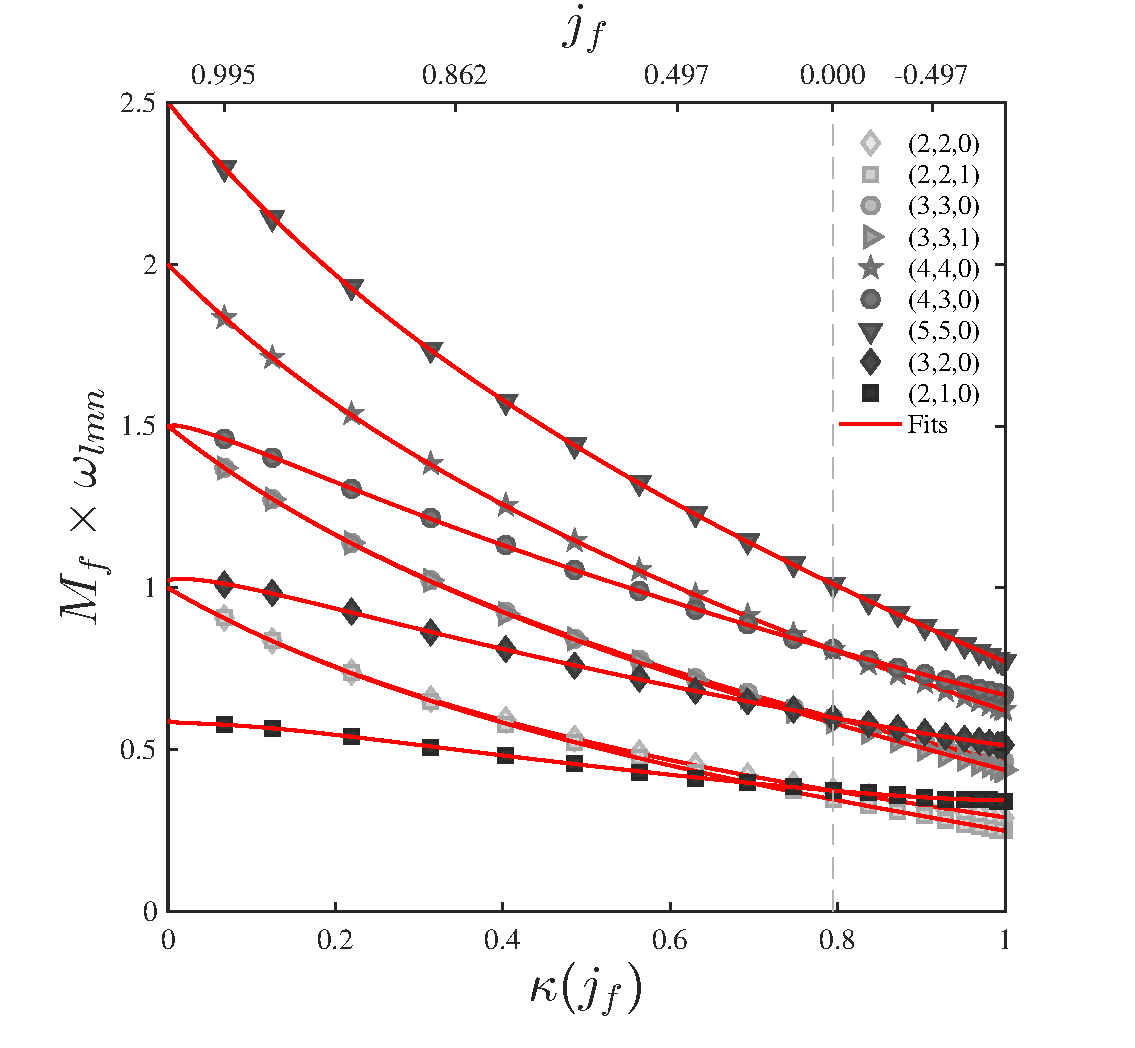
\includegraphics[width=\figfactor\textwidth]{fig/fits_w.pdf} & 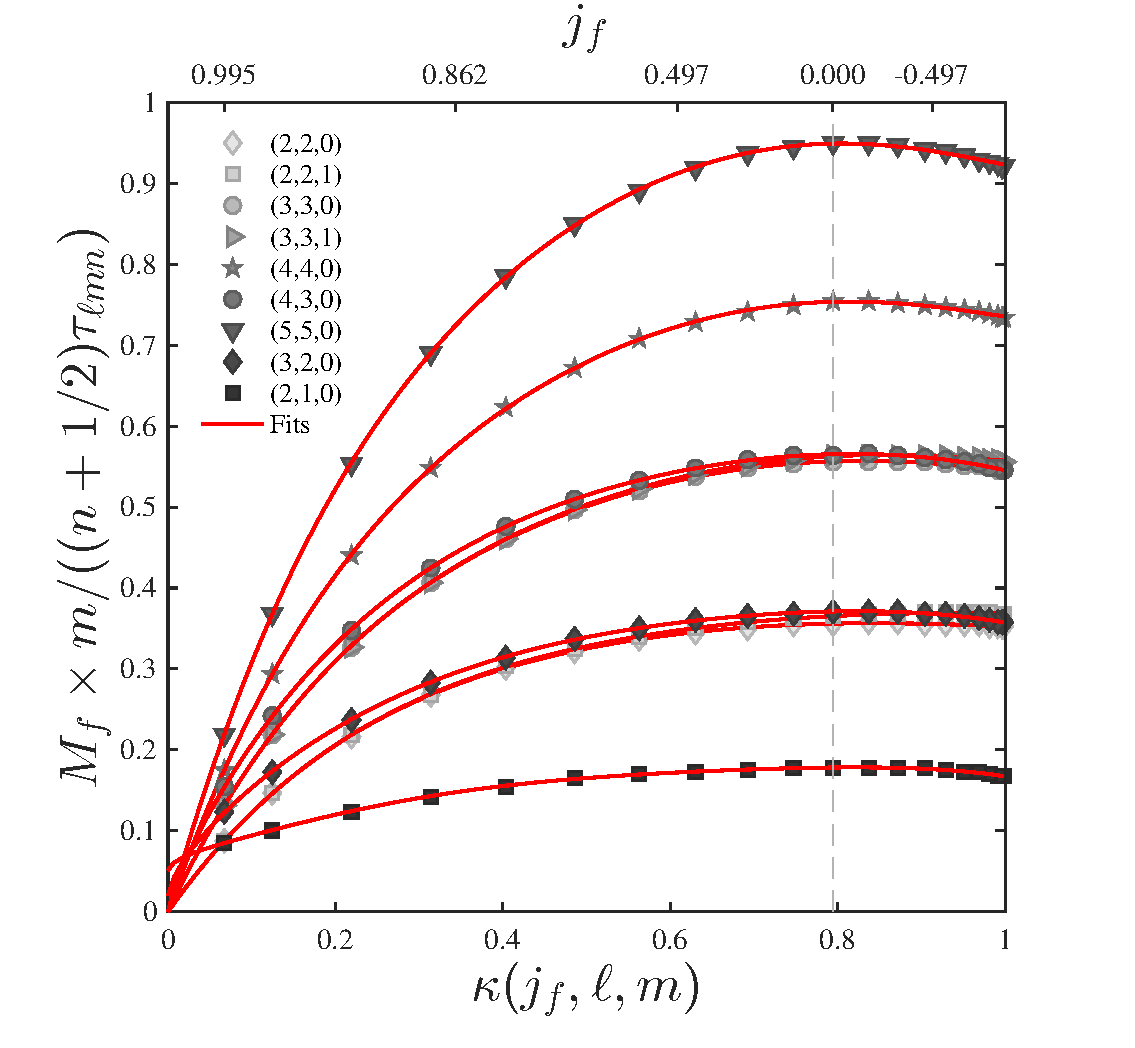
\includegraphics[width=\figfactor\textwidth]{fig/fits_tau.pdf}
  \end{tabular}
  %
	\caption{ Fits of dimensionless \qnm{} central frequencies (solid lines) along with select numerical values (grey markers) computed using Leaver's method \cite{Leaver85}.
  %
  Before the application of $\kappa(\j{})$, points are spaced between -\CwFitCalibrationRegion and \CwFitCalibrationRegion according to \CwFitCalibrationRegion times the $\sin$ of a fiducial angle which is uniformly spaced between $-\pi/2$ and $\pi/2$. Values of $\j{}$ are shown in the upper axis for $\kappa$ at $l=m$.
  %
  The grey dashed line marks the value of $\kappa$ where $\j{}=0$. Fits of dimensionless \qnm{} decay rates (solid lines) along with select numerical values (grey markers) computed using Leaver's method \cite{Leaver85}. }
  %
\end{figure*}

% Plots of mixing coefficients
\begin{figure*}
  %
  \begin{tabular}{lcr}
    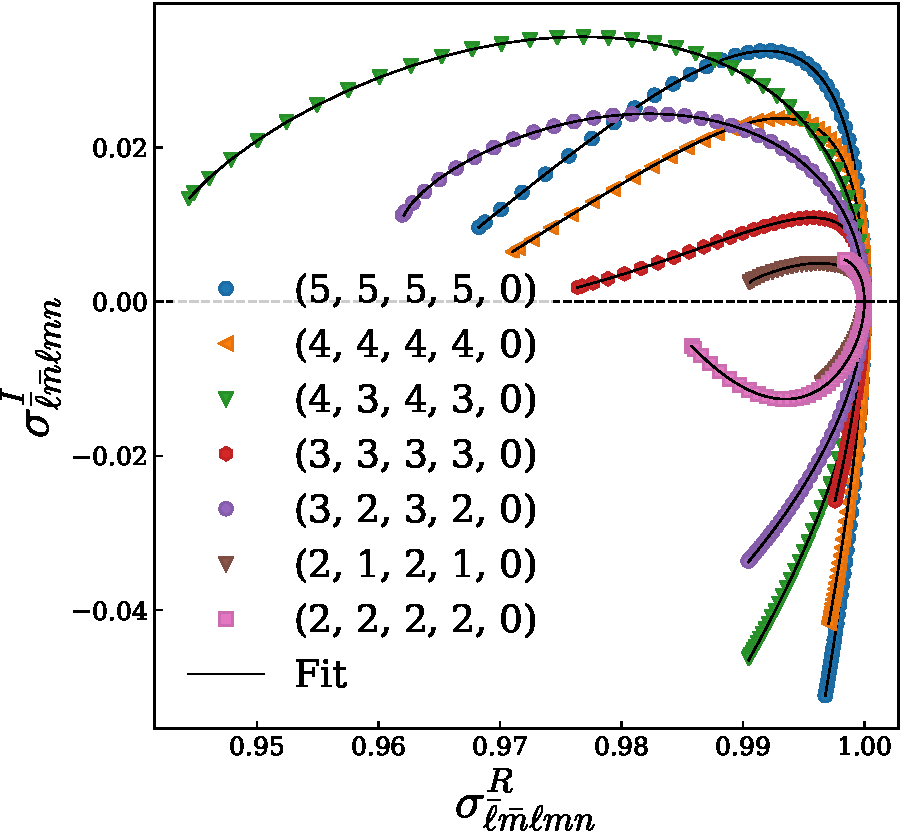
\includegraphics[width=\figfactor\textwidth]{fig/issue2_ysprod_1.pdf} & 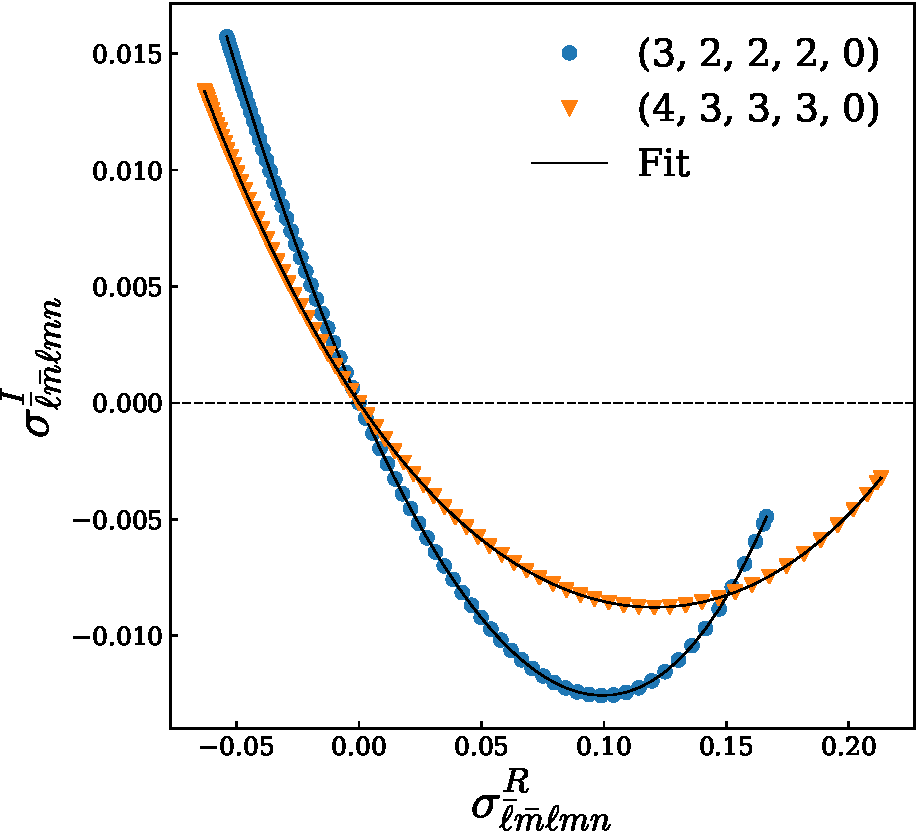
\includegraphics[width=\figfactor\textwidth]{fig/issue2_ysprod_2.pdf}
  \end{tabular}
  %
	\caption{ Spherical-spheroidal harmonic mixing coefficients. }
  %
\end{figure*}



%
\section{Discussion}
\label{discuss}

% %%%%%%%%%%%%%%%%%%%%%%%%%%%%%%%%%%%%%%%%%%%%%%%%% %
\bibliographystyle{ieeetr}
\bibliography{src/mvf.bib}
\end{document}
